\documentclass[crop,tikz,convert={outext=.svg,command=\unexpanded{pdf2svg \infile\space\outfile}},multi=false]{standalone}
\usepackage{tikz}
\usepackage{bm}
\usetikzlibrary{positioning}
\usetikzlibrary{decorations.pathreplacing}
\begin{document}

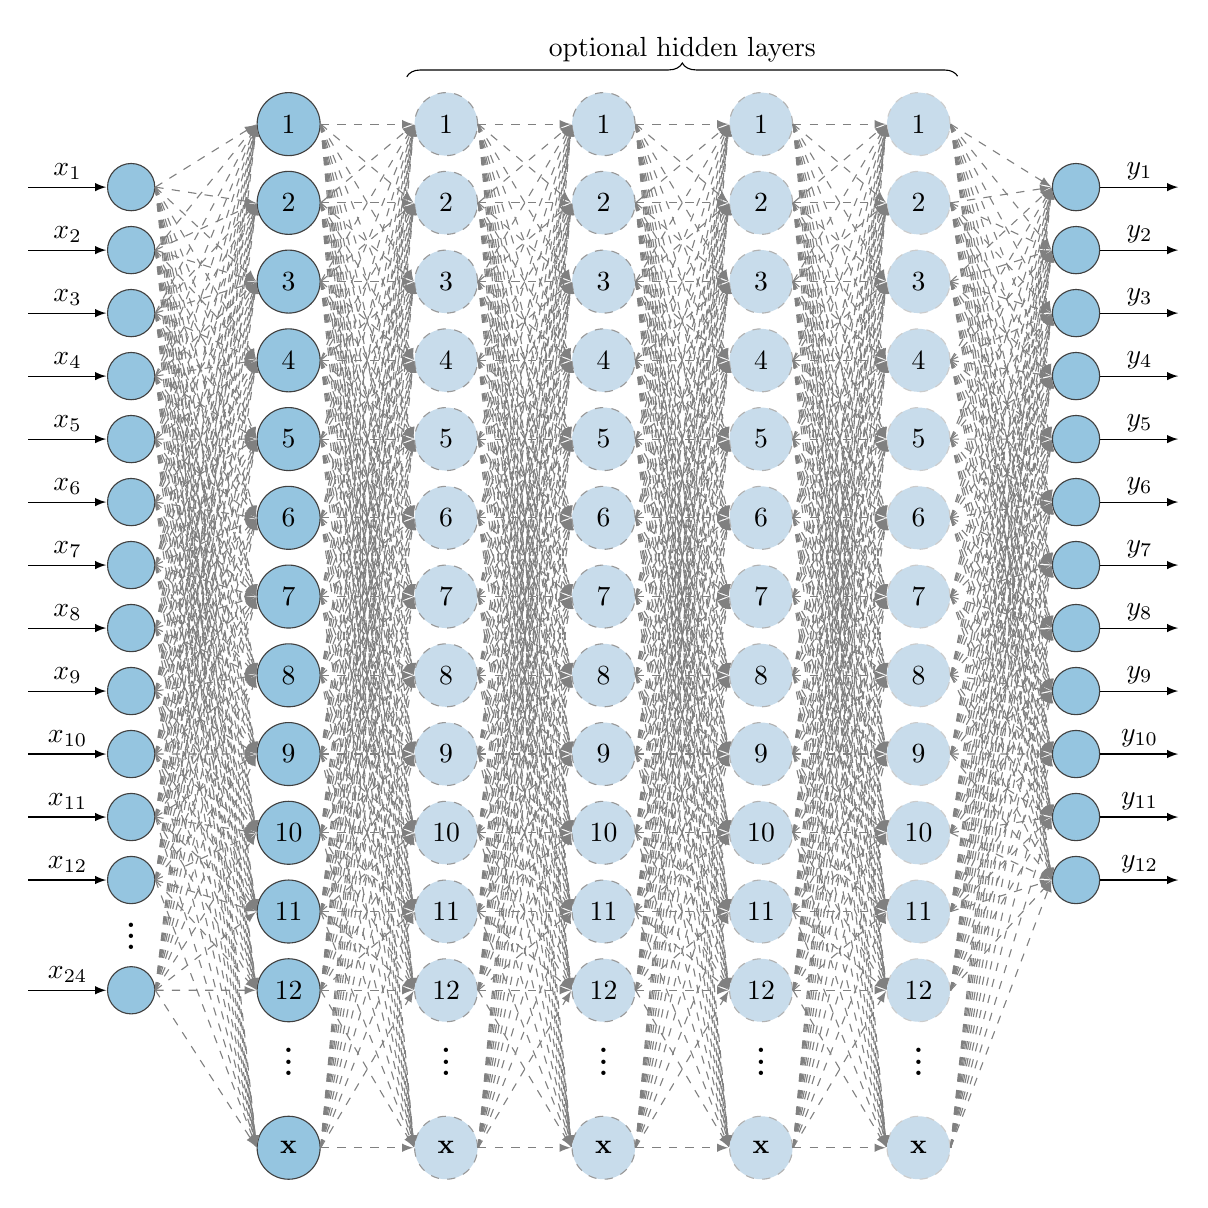
\begin{tikzpicture}[node distance=0.8cm and 0.8cm]
    \tikzset{every path/.style={shorten >=0.1mm}}
    
    % Farben
    \definecolor{Masch_light}{RGB}{149,197,224}
    \definecolor{Masch_faded}{RGB}{200,220,235}

    % Eingabeschicht (24 Neuronen)
    \foreach \i in {1,...,12} {
        \node[circle, draw=black!75,fill=Masch_light, minimum size=0.6cm] (input\i) at (0,-\i*0.8-1) {};
    }
    \node[circle, draw=black!75,fill=Masch_light, minimum size=0.6cm] (input13) at (0,-14*0.8-0.8) {};
    \node[align=center] ()[below=-0.1cm of input12] {$\bm{\vdots}$};

    % Optionaler Hidden Layer A (blass, gestrichelt)
    \foreach \i in {1,...,12} {
        \node[circle, draw=black!75,fill=Masch_light, minimum size=0.8cm] (hiddenA\i) at (2,-\i*1) {\i};
    }
    \node[circle, draw=black!75,fill=Masch_light, minimum size=0.8cm] (hiddenA13) at (2,-14*1) {\textbf{x}};
    \node[align=center] ()[below=-0cm of hiddenA12] {$\bm{\vdots}$};

    % Fokus: Hidden Layer B (voll dargestellt)
    \foreach \i in {1,...,12} {
        \node[circle, draw=black!40,dashed,fill=Masch_faded, minimum size=0.8cm] (hiddenB\i) at (4,-\i*1) {\i};
    }
    \node[circle, draw=black!40,dashed,fill=Masch_faded, minimum size=0.8cm] (hiddenB13) at (4,-14*1) {\textbf{x}};
    \node[align=center] ()[below=-0cm of hiddenB12] {$\bm{\vdots}$};

    % Optionaler Hidden Layer C (blass, gestrichelt)
    \foreach \i in {1,...,12} {
        \node[circle, draw=black!40,dashed,fill=Masch_faded, minimum size=0.8cm] (hiddenC\i) at (6,-\i*1) {\i};
    }
    \node[circle, draw=black!40,dashed,fill=Masch_faded, minimum size=0.8cm] (hiddenC13) at (6,-14*1) {\textbf{x}};
    \node[align=center] ()[below=-0cm of hiddenC12] {$\bm{\vdots}$};

    % Optionaler Hidden Layer D (blass, gestrichelt)
    \foreach \i in {1,...,12} {
        \node[circle, draw=black!30,dashed,fill=Masch_faded, minimum size=0.8cm] (hiddenD\i) at (8,-\i*1) {\i};
    }
    \node[circle, draw=black!30,dashed,fill=Masch_faded, minimum size=0.8cm] (hiddenD13) at (8,-14*1) {\textbf{x}};
    \node[align=center] ()[below=-0cm of hiddenD12] {$\bm{\vdots}$};

    % Optionaler Hidden Layer E (blass, gestrichelt)
    \foreach \i in {1,...,12} {
        \node[circle, draw=black!20,dashed,fill=Masch_faded, minimum size=0.8cm] (hiddenE\i) at (10,-\i*1) {\i};
    }
    \node[circle, draw=black!20,dashed,fill=Masch_faded, minimum size=0.8cm] (hiddenE13) at (10,-14*1) {\textbf{x}};
    \node[align=center] ()[below=-0cm of hiddenE12] {$\bm{\vdots}$};

    % Ausgabeschicht (12 Neuronen)
    \foreach \i in {1,...,12} {
        \node[circle, draw=black!75,fill=Masch_light, minimum size=0.6cm] (output\i) at (12,-\i*0.8-1) {};
    }

    % Verbindungen: Eingabe -> Hidden A (gestrichelt)
    \foreach \i in {1,...,13} {
        \foreach \j in {1,...,13} {
            \draw[-latex, dashed, draw=black!50] (input\i.east) -- (hiddenA\j.west);     
        }
    }

    % Hidden A -> Hidden B (gestrichelt)
    \foreach \i in {1,...,13} {
        \foreach \j in {1,...,13} {
            \draw[-latex, dashed, draw=black!50] (hiddenA\i.east) -- (hiddenB\j.west);
        }
    }

    % Hidden B -> Hidden C (gestrichelt)
    \foreach \i in {1,...,13} {
        \foreach \j in {1,...,13} {
            \draw[-latex, dashed, draw=black!50] (hiddenB\i.east) -- (hiddenC\j.west);
        }
    }

    % Hidden C -> Hidden D (gestrichelt)
    \foreach \i in {1,...,13} {
        \foreach \j in {1,...,13} {
            \draw[-latex, dashed, draw=black!50] (hiddenC\i.east) -- (hiddenD\j.west);
        }
    }

    % Hidden D -> Hidden E (gestrichelt)
    \foreach \i in {1,...,13} {
        \foreach \j in {1,...,13} {
            \draw[-latex, dashed, draw=black!50] (hiddenD\i.east) -- (hiddenE\j.west);
        }
    }

    % Hidden E -> Ausgabe (gestrichelt)
    \foreach \i in {1,...,13} {
        \foreach \j in {1,...,12} {
            \draw[-latex, dashed, draw=black!50] (hiddenE\i.east) -- (output\j.west);
        }
    }

    % Eingangs x-Beschriftungen
    \foreach \i in {1,...,12} {
        \draw[-latex] ([xshift=-1cm]input\i.west) -- node[yshift=0.2cm] {$x_{\i}$}(input\i.west);
    }
    \draw[-latex] ([xshift=-1cm]input13.west) -- node[yshift=0.2cm] {$x_{24}$}(input13.west);

    % Ausgangs y-Beschriftungen
    \foreach \i in {1,...,12} {
        \draw[-latex] (output\i.east) -- node[yshift=0.2cm] {$y_{\i}$}([xshift=1cm]output\i.east);
    }

    % Hinweistext für optionale Schichten
    \draw [decorate,decoration={brace,amplitude=5pt}]
  (3.5,-0.4) -- (10.5,-0.4) node[midway,yshift=1em]{optional hidden layers};

\end{tikzpicture}

\end{document}
